\documentclass[JCDReport.tex]{subfiles} 
\begin{document}

\subsection{Installation}

Fist, install the Git client of your preference \footnote{e.g. https://code.google.com/p/msysgit/}.\\

Then, start the command line, navigate to the folder where you would like to checkout the repository, and enter:\\
\textit{git clone git://github.com/lukaselmer/VFSPrototype.git}\\
Now, there should be a directory VFSPrototype. In the further installation instructions, the path to this folder will be referenced as \textit{repository checkout location}.\\

Before the project can be started, the following software has to be installed. Even tough the software could run on other configurations too, there is no guarantee that the software will run (correctly) with a different configuration.

\begin{enumerate}
\item Windows 8 Professional, 64 Bit
\item Visual Studio 2012 Ultimate Edition (VS2012)
\item NuGet packet manager addon\footnote{http://visualstudiogallery.msdn.microsoft.com/27077b70-9dad-4c64-adcf-c7cf6bc9970c} for VS2012 (restart VS2012 after installing the addon)
\end{enumerate}

Additionally, it is required to add the folder that contains sqlite.dll to the system path. This folder is (relative to the Git repository root): "\textit{repository checkout location}/Code/VFSPrototype/sqlite/". After this, \textbf{your pc has to be restarted}, otherwise it will probably not work.\\
In case you would not like to add this directory to the system path, you can copy the sqlite.dll and the sqlite.def to the Windows/System32 directory.\\

Then, after installing the sqlite.dll and the NuGet packet manager addon, open the solution at "\textit{repository checkout location}/Code/VFSPrototype/VFSPrototype.sln". After the project is loaded, right click on the solution and click on "Enable NuGet Package Restore", see Figure \ref{fig:nugetPackageRestore} on page \pageref{fig:nugetPackageRestore}. If this button is not available, then the NuGet package manager probably is not installed correctly.\\

\begin{figure}[h!]
	\centering
	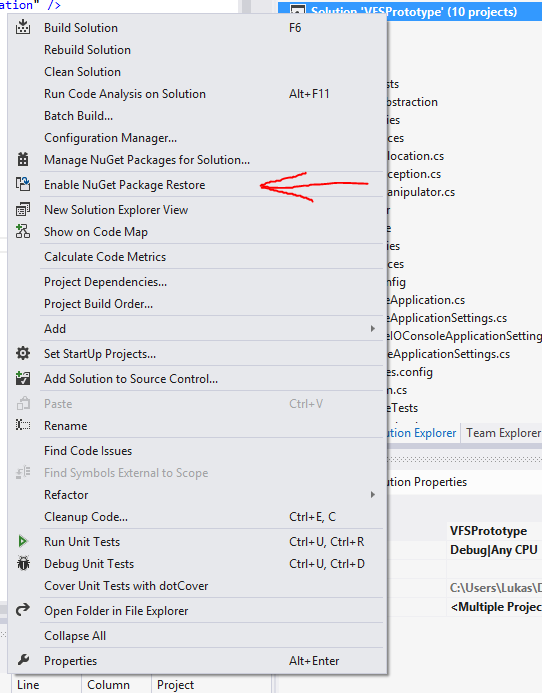
\includegraphics[scale=1]{Images/nuget_restore.png} 
	\caption{EnableNuGet Package Restore}
	\label{fig:nugetPackageRestore}
\end{figure}	

To start the server, right click on the project "VFSWCFContracts", click "Debug"/"Start new instance". Now the server should be running and a new browser window should open.\\

To start the client, right click on the project "Startup", click "Debug"/"Start new instance". Now the client should be running and a new window with the file system browser should open.\\

You can start as many clients a you would like.\\

There is one more catch, literally. Try the login functionality with some wrong credentials. Now the VS2012 will witch to the debug mode, because a FaultException was thrown. This is inconvenient, because these exceptions are propagated to the client, because of the FaultContracts. To disable this behaviour, stop the program, and click on "Debug"/"Exceptions" in the VS2012 main menu bar. Then a new window should occur. Click on "Find..." and enter "FaultException". You should find two items "FaultException" and "FaultException'1". Disable all flags of these two exceptions, especially the "User-unhandled" checkbox. Press ok, and you will not see this exception again.


\subsection{Console Application}

% If you have a command line interface for your VFS, describe here the commands available (e.g. ls, copy, import).

The console application was developed at the beginning of the project. Therefore, many options available in the GUI are not available in the console.\\

Available commands:
\begin{itemize}
\item cd
\item delete
\item exists
\item exit
\item export
\item help
\item import
\item ls
\item mkdir
\end{itemize}



\subsection{Scenario}

% TODO: Remove this text and replace it with actual content
% Describe how to realize the following use case with your system. Describe the steps involved and how to perform each action (e.g. command line executions and arguments, menu entries, keyboard shortcuts, screenshots). The use case is the following:
%\begin{enumerate}
%\item Start synchronization server on localhost.
%\item Create account on synchronization server.
%\item Create two VFS disks (on the same machine) and link them to the new account.
%\item Import a directory (recursively) from the host file system into Disk 1.
%\item Dispose Disk 1 after the synchronization finished.
%\item Export the directory (recursively) from Disk 2 into the host file system.
%\item Stop synchronization server.
%\end{enumerate}
%}


\begin{figure}[h!]
	\centering
	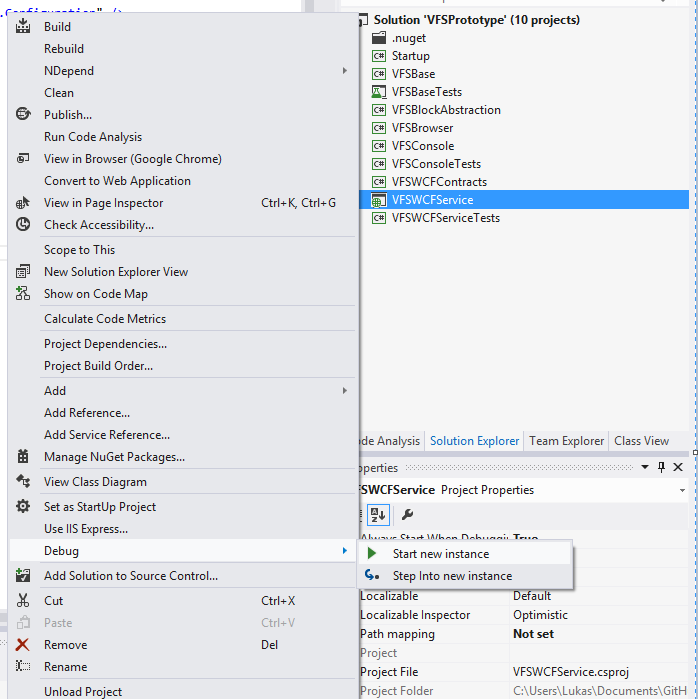
\includegraphics[scale=0.75]{Images/tutorial/1.png} 
	\caption{synchronization server on localhost.}
\end{figure}	

\begin{figure}[h!]
	\centering
	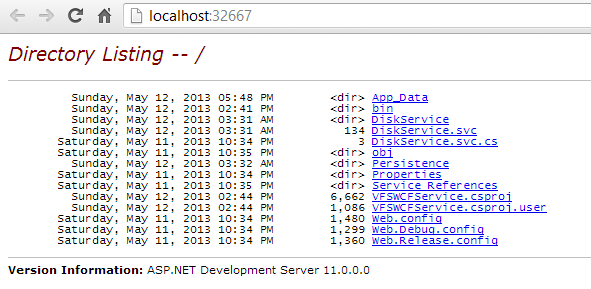
\includegraphics[scale=0.75]{Images/tutorial/2.png} 
	\caption{You should see this.}
\end{figure}

\begin{figure}[h!]
	\centering
	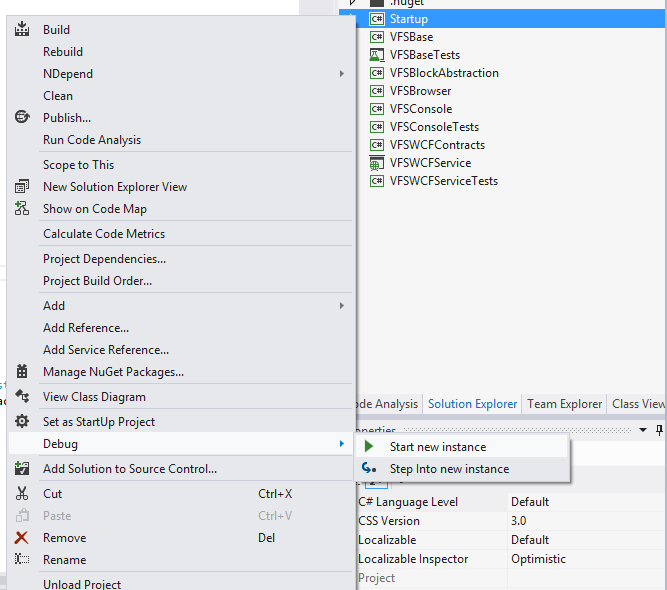
\includegraphics[scale=0.75]{Images/tutorial/3.png} 
	\caption{Start the client (do this two times to start two clients).}
\end{figure}

\begin{figure}[h!]
	\centering
	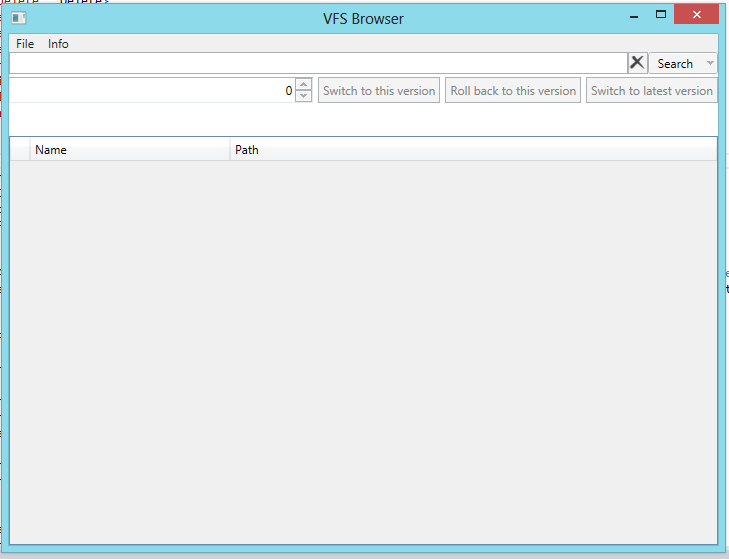
\includegraphics[scale=0.75]{Images/tutorial/4.png} 
	\caption{You should see this (two times if the client has been started two times).}
\end{figure}

\begin{figure}[h!]
	\centering
	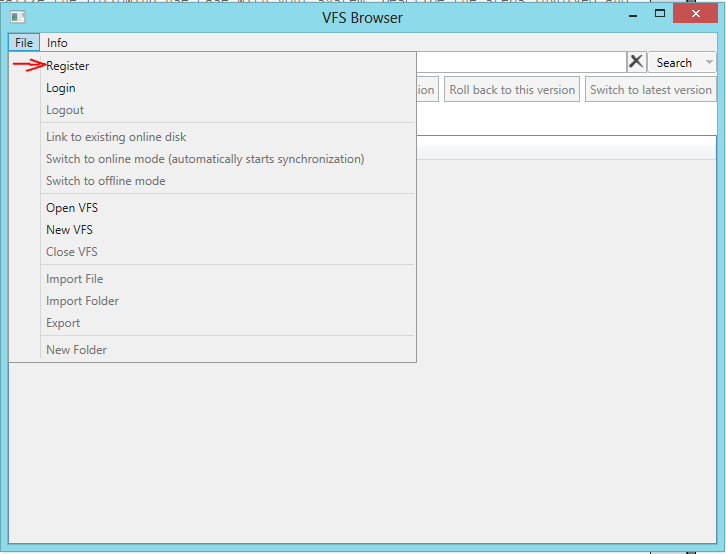
\includegraphics[scale=0.75]{Images/tutorial/5.png} 
	\caption{Register a new user account.}
\end{figure}

\begin{figure}[h!]
	\centering
	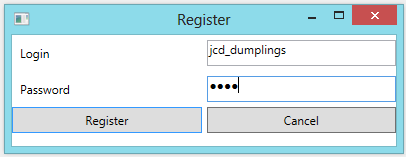
\includegraphics[scale=1]{Images/tutorial/6.png} 
	\caption{Enter credentials.}
\end{figure}

\begin{figure}[h!]
	\centering
	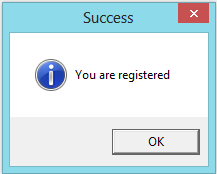
\includegraphics[scale=1]{Images/tutorial/7.png} 
	\caption{Registration successful.}
\end{figure}

\begin{figure}[h!]
	\centering
	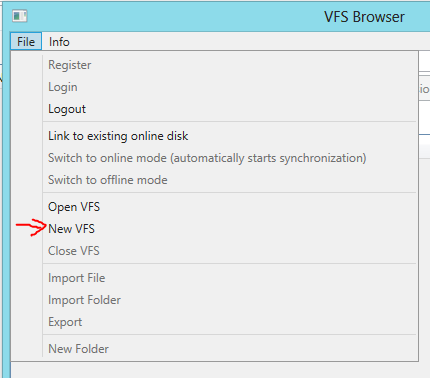
\includegraphics[scale=1]{Images/tutorial/8.png} 
	\caption{Create a new (local) VFS.}
\end{figure}

\begin{figure}[h!]
	\centering
	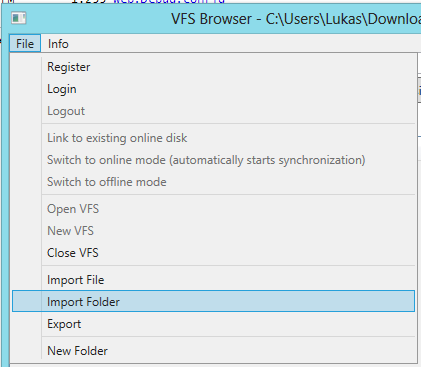
\includegraphics[scale=1]{Images/tutorial/8_2.png} 
	\caption{Import any folder.}
\end{figure}

\begin{figure}[h!]
	\centering
	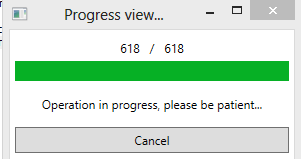
\includegraphics[scale=1]{Images/tutorial/9.png} 
	\caption{You should see the progress bar from the import.}
\end{figure}

\begin{figure}[h!]
	\centering
	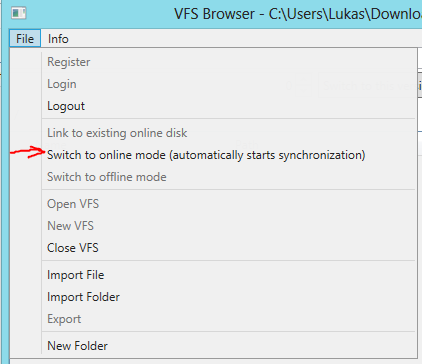
\includegraphics[scale=1]{Images/tutorial/10.png} 
	\caption{Switch to online mode to start synchronization.}
\end{figure}

\begin{figure}[h!]
	\centering
	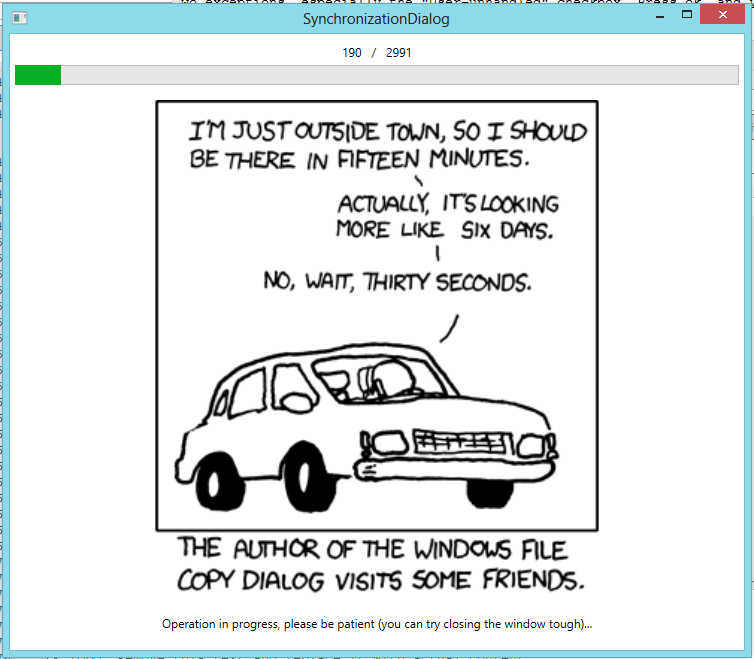
\includegraphics[scale=0.75]{Images/tutorial/11.png} 
	\caption{When the synchronization starts, you should see this dialogue.}
\end{figure}

\begin{figure}[h!]
	\centering
	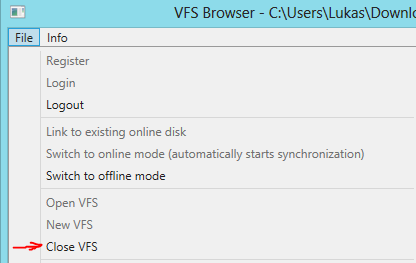
\includegraphics[scale=1]{Images/tutorial/15.png} 
	\caption{Close the VFS.}
\end{figure}

\begin{figure}[h!]
	\centering
	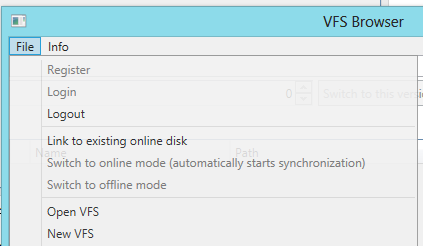
\includegraphics[scale=1]{Images/tutorial/12.png} 
	\caption{Switch to the other client, login with your credentials, and choose Link to existing disk.}
\end{figure}

\begin{figure}[h!]
	\centering
	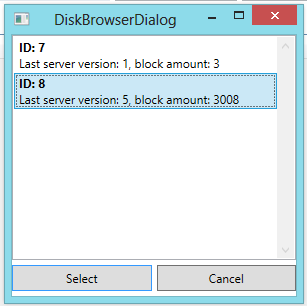
\includegraphics[scale=1]{Images/tutorial/13.png} 
	\caption{Select a disk.}
\end{figure}

\begin{figure}[h!]
	\centering
	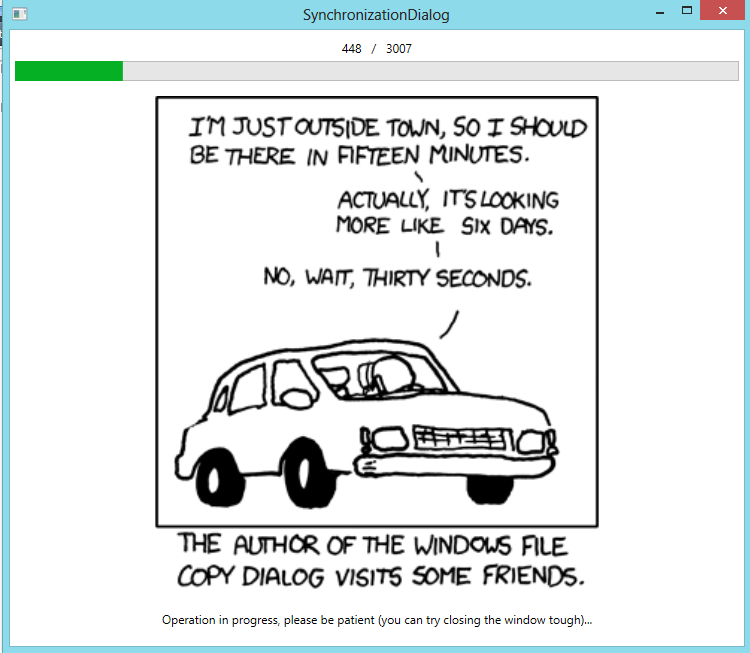
\includegraphics[scale=0.75]{Images/tutorial/14.png} 
	\caption{When switching to online mode again, you should see the synchronization dialogue.}
\end{figure}

\begin{figure}[h!]
	\centering
	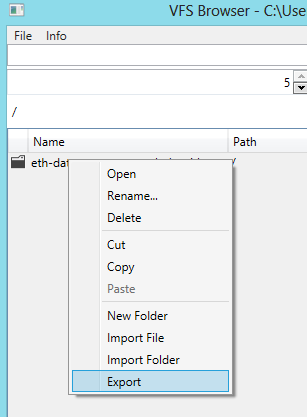
\includegraphics[scale=1]{Images/tutorial/16.png} 
	\caption{As soon as the dialogue is closed, right click on the synchronized folder to export it.}
\end{figure}

\begin{figure}[h!]
	\centering
	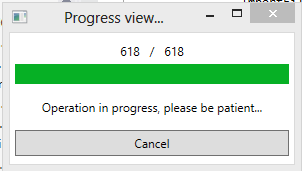
\includegraphics[scale=1]{Images/tutorial/17.png} 
	\caption{Once again, a progress report shows the export progress. After the export has finished, the folder you imported now is on the host system.}
\end{figure}



\end{document}
